% ═══════════════════════════════════════════════════════════════════════════
% Chapter 8: Rep Segmentation Algorithm
% ═══════════════════════════════════════════════════════════════════════════

\chapter{Real-Time Rep Segmentation} \label{chap:segmentation}

\section{Problem Formulation}

Rep segmentation identifies the temporal boundaries of individual repetition cycles and computes kinematic metrics for each phase. The algorithm must operate in real-time with bounded latency while maintaining accuracy against optical ground truth.

\section{Rep Phase Definitions}

A complete repetition comprises four sequential phases:

\begin{figure}[h]
    \centering
    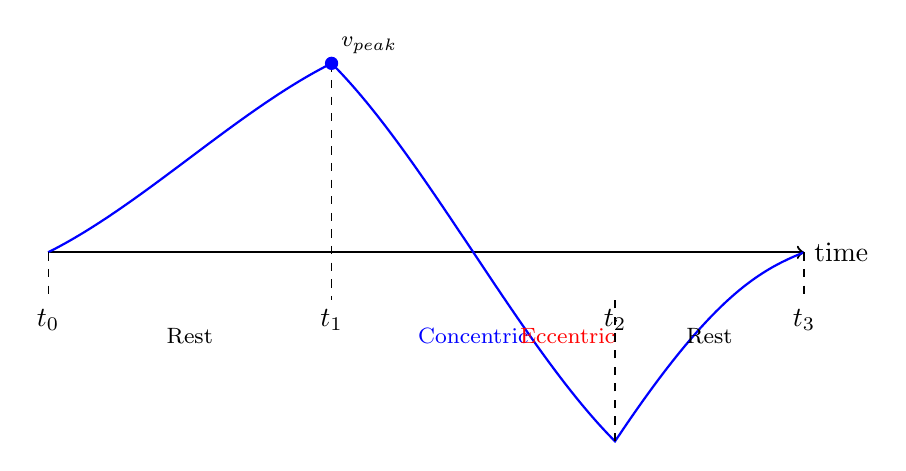
\begin{tikzpicture}[scale=1.2]
        % Time axis
        \draw[->, thick] (0,0) -- (8,0) node[right] {time};

        % Velocity trace
        \draw[thick, blue] (0,0) .. controls (1,0.5) and (2,1.5) .. (3,2)
                               .. controls (4,1) and (5,-1) .. (6,-2)
                               .. controls (7,-0.5) and (7.5,-0.2) .. (8,0);

        % Phase boundaries
        \draw[dashed] (0,0) -- (0,-0.5) node[below] {$t_0$};
        \draw[dashed] (3,2) -- (3,-0.5) node[below] {$t_1$};
        \draw[dashed] (6,-2) -- (6,-0.5) node[below] {$t_2$};
        \draw[dashed] (8,0) -- (8,-0.5) node[below] {$t_3$};

        % Phase labels
        \node[below, font=\footnotesize] at (1.5,-0.7) {Rest};
        \node[below, font=\footnotesize, blue] at (4.5,-0.7) {Concentric};
        \node[below, font=\footnotesize, red] at (5.5,-0.7) {Eccentric};
        \node[below, font=\footnotesize] at (7,-0.7) {Rest};

        % Peak velocity marker
        \fill[blue] (3,2) circle (2pt);
        \node[above right, font=\footnotesize] at (3,2) {$v_{peak}$};
    \end{tikzpicture}
    \caption{Rep phase decomposition with velocity trace}
    \label{fig:rep_phases}
\end{figure}

\begin{enumerate}
    \item \textbf{Rest ($t_0$ to $t_1$):} Barbell stationary at starting position
    \item \textbf{Concentric ($t_1$ to $t_2$):} Lifting phase, positive velocity
    \item \textbf{Eccentric ($t_2$ to $t_3$):} Lowering phase, negative velocity
    \item \textbf{Rest ($t_3$ onwards):} Barbell stationary at ending position
\end{enumerate}

\section{Dual-Trigger Boundary Detection}

\subsection{Trigger 1: Stillness Confirmation}

For exercises with inter-rep rests (deadlift, squat), stillness detection provides precise boundaries:

\begin{lstlisting}[language=python]
def is_still(accel_window, gyro_window, config):
    """Check if barbell is stationary."""
    accel_std = np.std(np.linalg.norm(accel_window, axis=1))
    gyro_rms = np.sqrt(np.mean(np.sum(gyro_window**2, axis=1)))

    return (accel_std < config.still_acc_band_g and
            gyro_rms < config.still_gyr_dps and
            len(accel_window) >= config.still_min_samples)
\end{lstlisting}

\subsection{Trigger 2: Windowed Extremum}

For continuous-rep exercises (bench press, barbell row), velocity zero-crossing via position extremum detection:

\begin{equation}
    t_{top} = \arg\max_{\tau \in [t-W, t+W]} p(\tau) \quad \text{subject to} \quad
    p(\tau) - \min_{u \in [\tau-W, \tau+W]} p(u) > \text{prominence}
\end{equation}

\begin{equation}
    t_{bottom} = \arg\min_{\tau \in [t-W, t+W]} p(\tau) \quad \text{subject to} \quad
    \max_{u \in [\tau-W, \tau+W]} p(u) - p(\tau) > \text{prominence}
\end{equation}

\subsection{Back-Dating Strategy}

The extremum detection inherently lags the true boundary by $\approx 200$ ms. We back-date to the minimum-motion sample:

\begin{figure}[h]
    \centering
    \begin{tikzpicture}[scale=1]
        \draw[->, thick] (0,0) -- (10,0) node[right] {time};
        \draw[->, thick] (0,-3) -- (0,3) node[above] {motion};

        % Motion trace
        \draw[thick, red] (0,0.5) .. controls (2,0.8) and (4,2.5) .. (5,2.8)
                                   .. controls (6,1.5) and (7,0.3) .. (8,0.1)
                                   .. controls (9,0.05) and (9.5,0.02) .. (10,0.2);

        \draw[dashed, ->] (7,2.5) node[right] {Detected boundary} -- (7,0);
        \draw[dashed, ->] (8.5,2) node[right] {Back-dated boundary} -- (8.5,0);

        \node[below, font=\footnotesize] at (8.5,0) {$t_{true}$};
    \end{tikzpicture}
    \caption{Back-dating from detected to true boundary}
    \label{fig:backdating}
\end{figure}

\section{Per-Rep Metrics Computation}

\subsection{Concentric Phase Metrics}

\begin{align}
    v_{peak,\text{con}} &= \max_{t \in [t_1, t_2]} v(t) \\
    \bar{v}_{\text{con}} &= \frac{1}{t_2 - t_1} \int_{t_1}^{t_2} v(t) \, dt \\
    \text{ROM}_{\text{vertical}} &= p(t_2) - p(t_1)
\end{align}

\subsection{Eccentric Phase Metrics}

\begin{align}
    v_{peak,\text{ecc}} &= \min_{t \in [t_2, t_3]} v(t) \quad (\text{negative value}) \\
    \bar{v}_{\text{ecc}} &= \frac{1}{t_3 - t_2} \int_{t_2}^{t_3} v(t) \, dt
\end{align}

\subsection{3D Bounding Box ROM}

For technique analysis, we compute the full 3D displacement:

\begin{equation}
    \text{ROM}_{3D} = \sqrt{(x_{\max} - x_{\min})^2 + (y_{\max} - y_{\min})^2 + (z_{\max} - z_{\min})^2}
\end{equation}

\section{Set-Level Aggregation}

\subsection{Intra-Set Velocity Loss}

\begin{equation}
    \%VL = 100 \cdot \left(1 - \frac{\bar{v}_{\text{last}}}{\bar{v}_{\text{first}}}\right)
\end{equation}

\subsection{Set-Average Metrics}

\begin{align}
    \bar{v}_{\text{set}} &= \frac{1}{N} \sum_{i=1}^{N} \bar{v}_{\text{con}, i} \\
    \text{ROM}_{\text{set}} &= \frac{1}{N} \sum_{i=1}^{N} \text{ROM}_{\text{vertical}, i} \\
    T_{\text{summary}} &= \sum_{i=1}^{N} (t_{2,i} - t_{1,i}) \quad \text{(time under tension)}
\end{align}

\section{Exercise-Specific Adaptations}

\subsection{Deadlift}

Deadlift features distinct top and bottom rests. The stillness trigger fires at both boundaries:

\begin{table}[h]
    \centering
    \caption{Deadlift phase detection}
    \begin{tabular}{ll}
        \toprule
        \textbf{Boundary} & \textbf{Trigger} \\
        \midrule
        Rep start (bottom) & Stillness after floor contact \\
        Rep end (top) & Stillness at lockout \\
        \bottomrule
    \end{tabular}
\end{table}

\subsection{Bench Press}

Bench press often uses continuous reps without top rest. The extremum trigger fires at chest touch and bar lift-off:

\begin{table}[h]
    \centering
    \caption{Bench press phase detection}
    \begin{tabular}{ll}
        \toprule
        \textbf{Boundary} & \textbf{Trigger} \\
        \midrule
        Rep start (top) & Position minimum at chest \\
        Rep end (bottom) & Position maximum at lockout \\
        \bottomrule
    \end{tabular}
\end{table}

\subsection{Snatch}

Snatch features rapid transitions and potential multi-phase pulls. We employ tighter gates:

\begin{align}
    \text{still\_min\_s} &= 50 \text{ ms} \quad \text{(vs. 80 ms default)} \\
    \text{peak\_window\_s} &= 150 \text{ ms} \quad \text{(vs. 220 ms default)}
\end{align}

\section{Manual Annotation Override}

\subsection{Annotation Interface}

The GUI provides manual boundary adjustment for validation dataset curation:

\begin{itemize}
    \item Drag phase boundary markers on the velocity trace
    \item Insert/delete rep boundaries
    \item Merge adjacent reps (for split detections)
    \item Split single rep into multiple phases
\end{itemize}

\subsection{Annotation Quality Control}

Each annotation queue entry displays:
\begin{itemize}
    \item Video synchronized to signal timestamps
    \item Acceleration and gyro traces
    \item Computed velocity and position
    \item Previous annotation history (if available)
\end{itemize}

\section{Latency Analysis}

\begin{table}[h]
    \centering
    \caption{Segmentation latency breakdown}
    \label{tab:seg_latency}
    \begin{tabular}{lr}
        \toprule
        \textbf{Component} & \textbf{Latency} \\
        \midrule
        Stillness gate (80 ms hold) & 80 ms \\
        Extremum detection (220 ms window) & 220 ms \\
        Back-dating search (300 ms window) & $<$1 ms \\
        Per-rep batch smoothing & $\approx$5 ms \\
        \midrule
        \textbf{Total (stillness trigger)} & \textbf{$\approx$88 ms} \\
        \textbf{Total (extremum trigger)} & \textbf{$\approx$228 ms} \\
        \bottomrule
    \end{tabular}
\end{table}

Both triggers meet the 500 ms latency budget with substantial margin.

\section{Summary}

This chapter presented the real-time rep segmentation algorithm with dual-trigger boundary detection, back-dating strategy, and per-rep metrics computation. The algorithm achieves $<$300 ms latency for all repetition types while maintaining $>$90\% F1 score against manual annotations (see \Cref{chap:validation}).

\newpage